\section{Results} \label{sec:results}
In this section, I present the result Android app that is developed. The app follows the requirement and use cases which are analyzed in section \textbf{section \ref{sec:usecase}}. At first, I show interfaces of some main activities of the app. After that, the performance of the app is reported. In the second half of this section, I report the accuracy of the hair and clothes segmentation model, which is already proposed in \textbf{section \ref{sec:model}}. 

\subsection{Android app}
\subsubsection{User interface}
An Android app is comprised of one or more activities, meaning one or more screens. Each activity is one screen of that app's user interface. The Android app starts by showing the main activity, and from there, the app may make it possible to open other activities. Here is some core activities of the app:
\begin{itemize}
    \item Main Activity
    \item Color Scanning Activity
    \item Camera Activity
    \item Segmentation Activity
    \item Post-capture Activity
\end{itemize}
The following are screenshots of these activities.

\begin{figure} [H]
    \centering
    \captionsetup{justification=centering}
    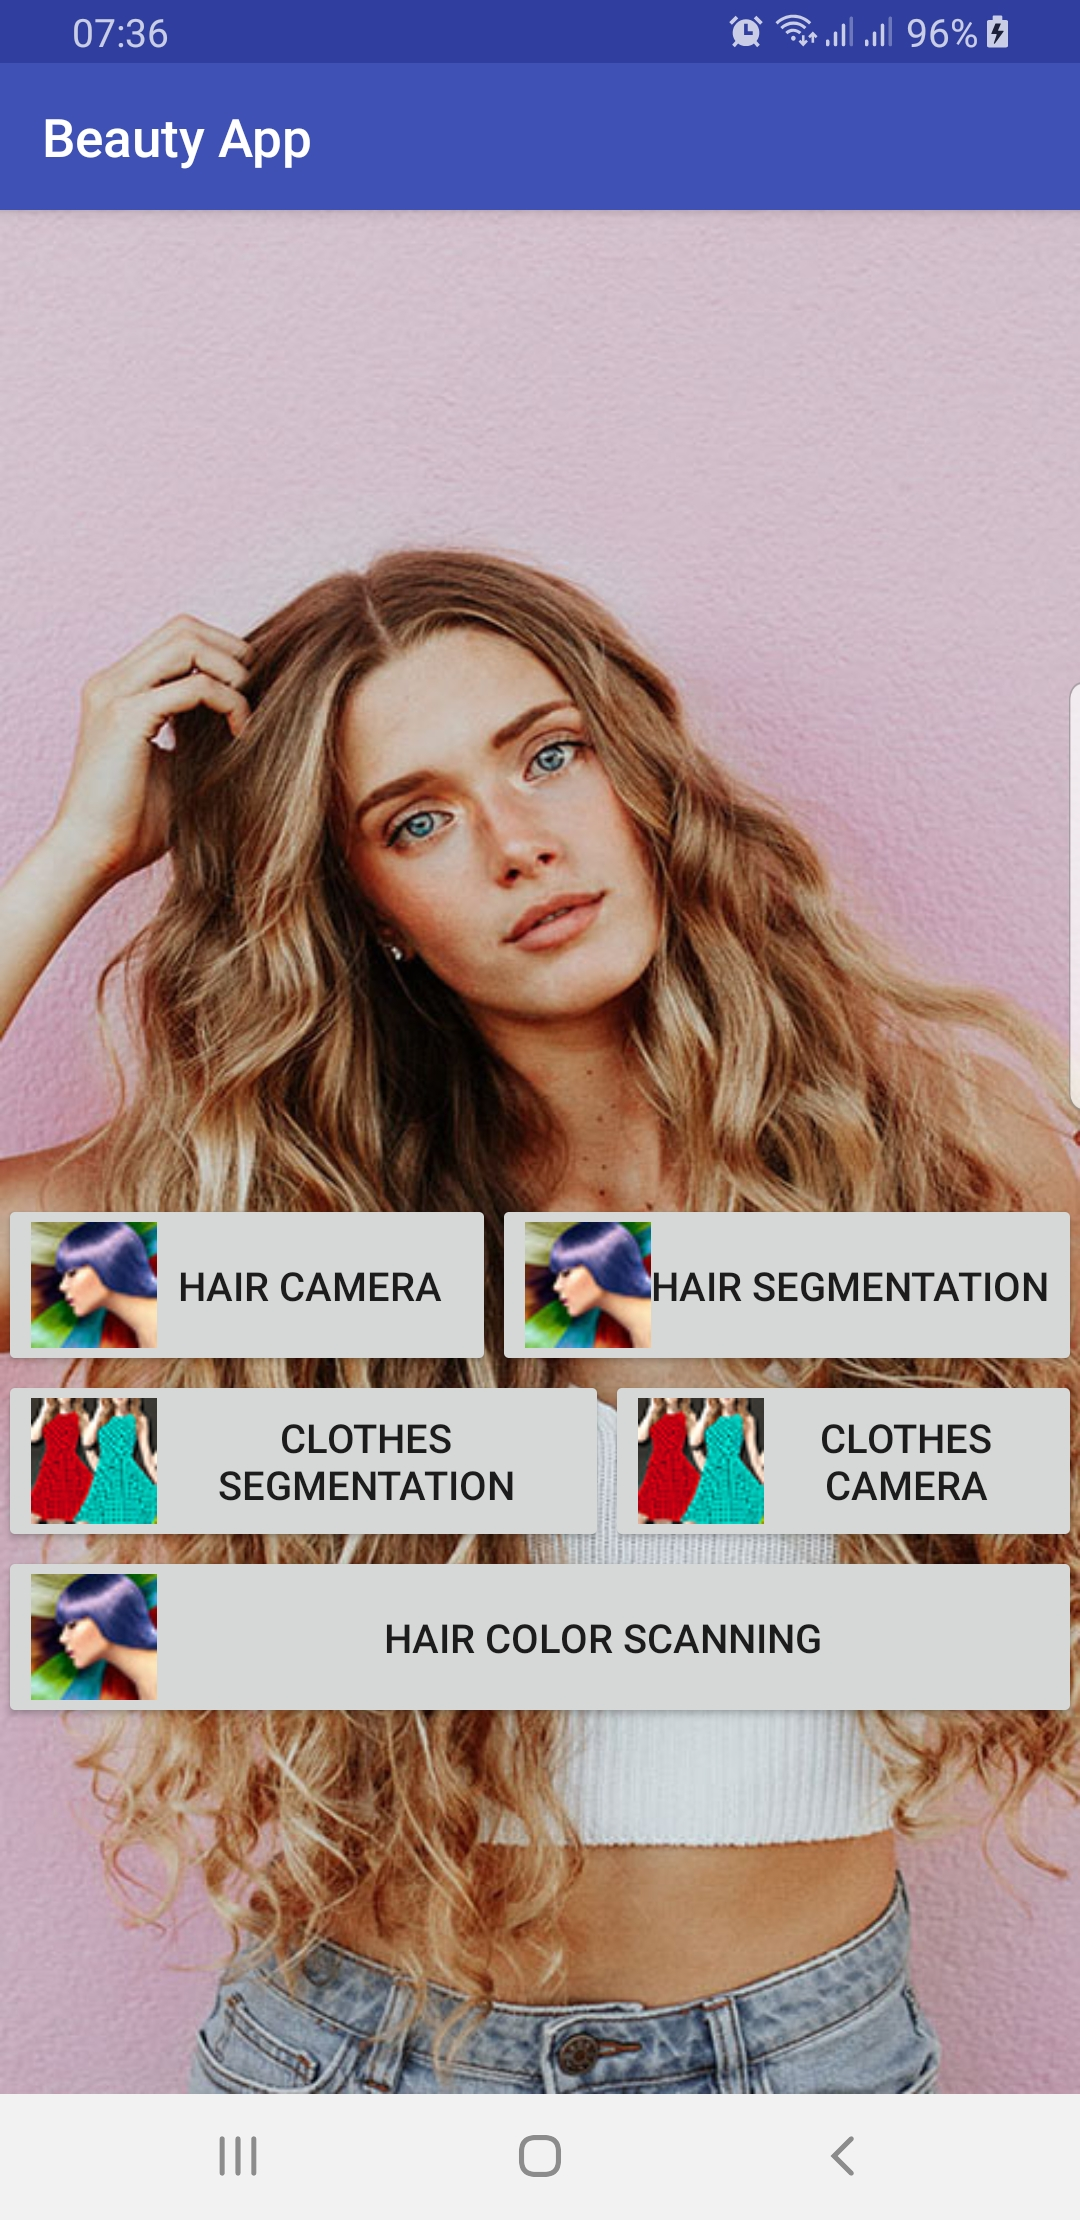
\includegraphics[width=0.3\textwidth]{chapter4/image/home.jpg}
    \caption{Illustration for Main Activity}
\end{figure}

\begin{figure} [H]
    \centering
    \captionsetup{justification=centering}
    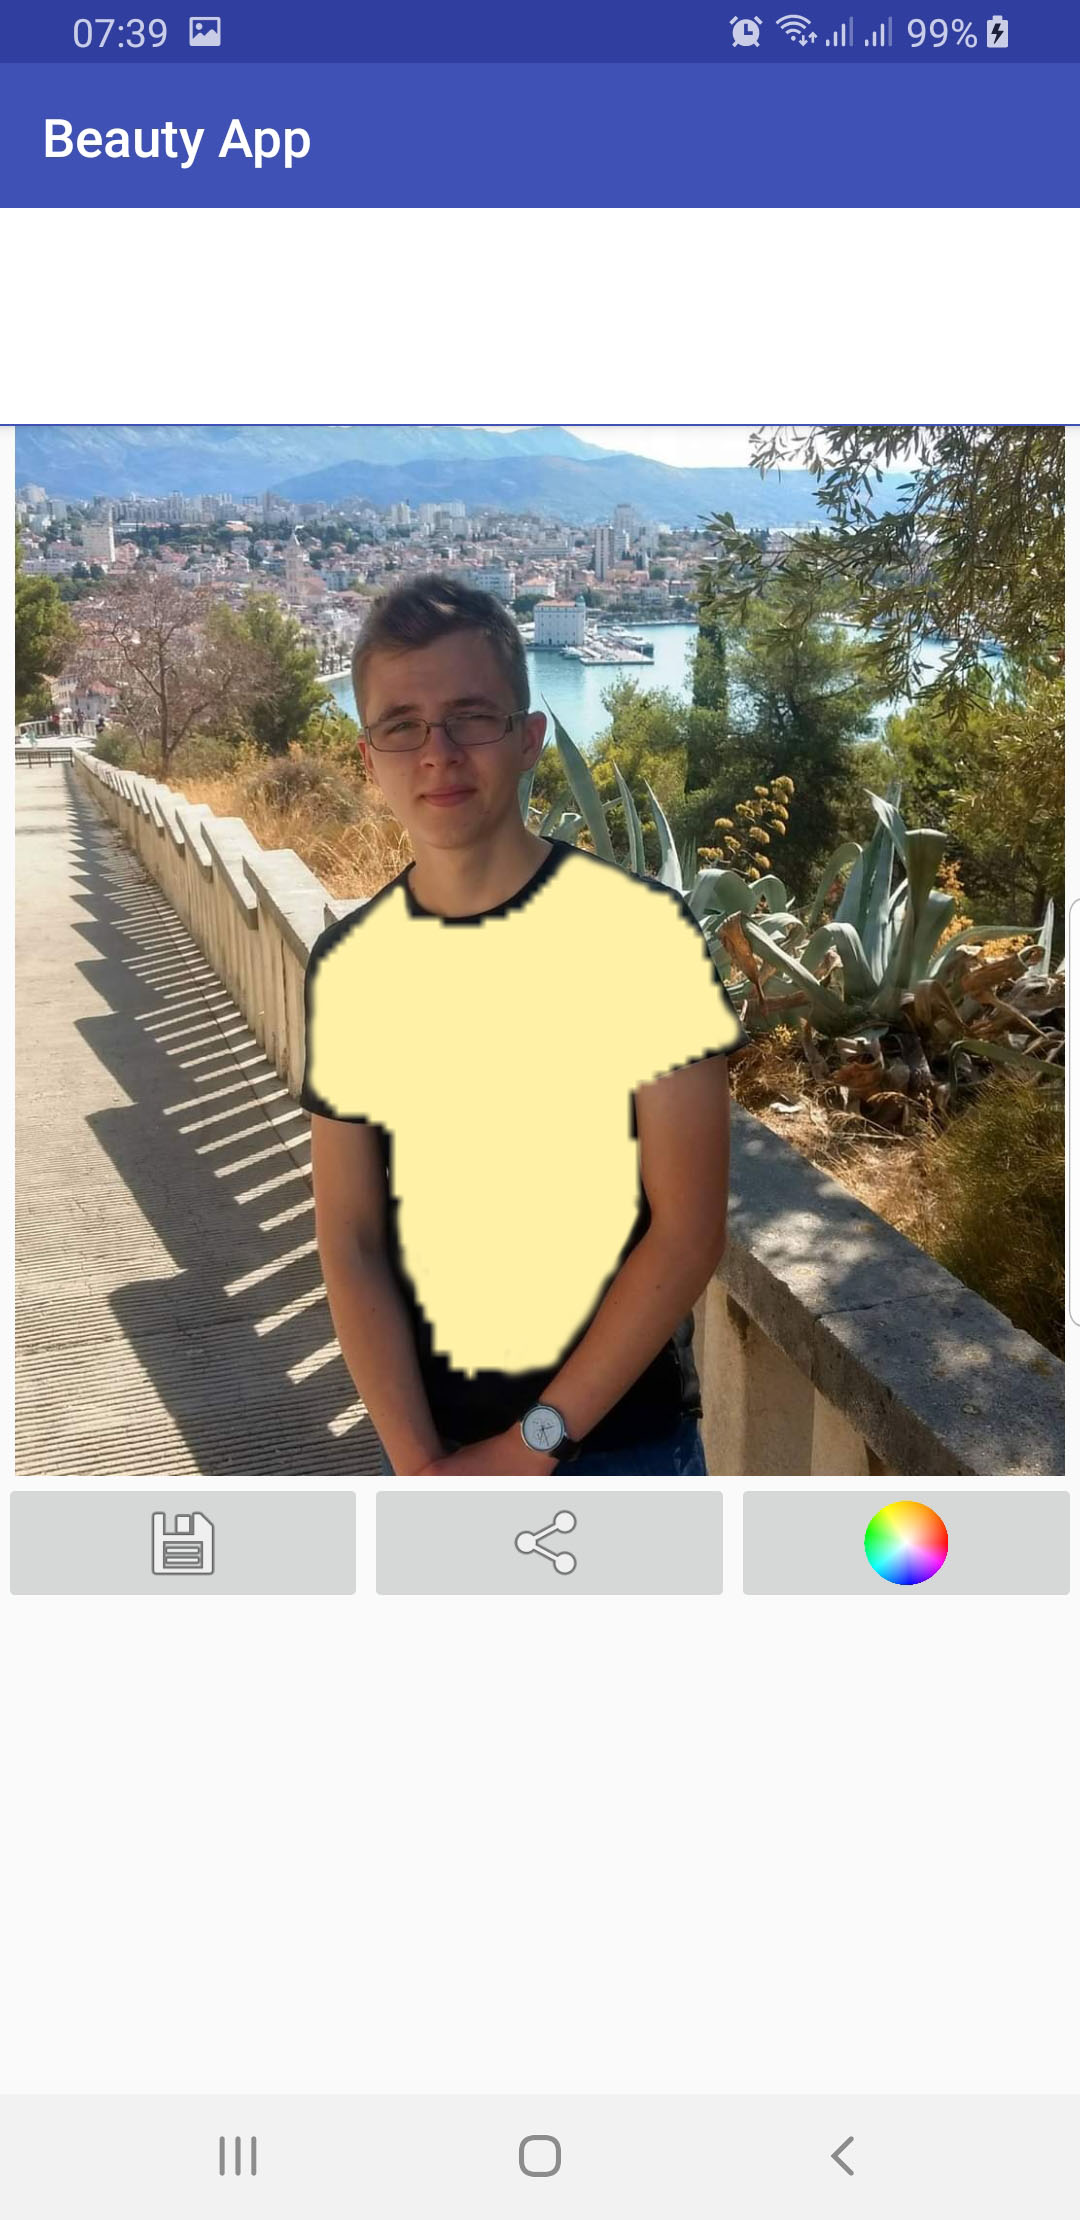
\includegraphics[width=0.3\textwidth]{chapter4/image/segment.jpg}
    \caption{Illustration for Clothes Segmentation Activity}
\end{figure}

\begin{figure} [H]
    \centering
    \captionsetup{justification=centering}
    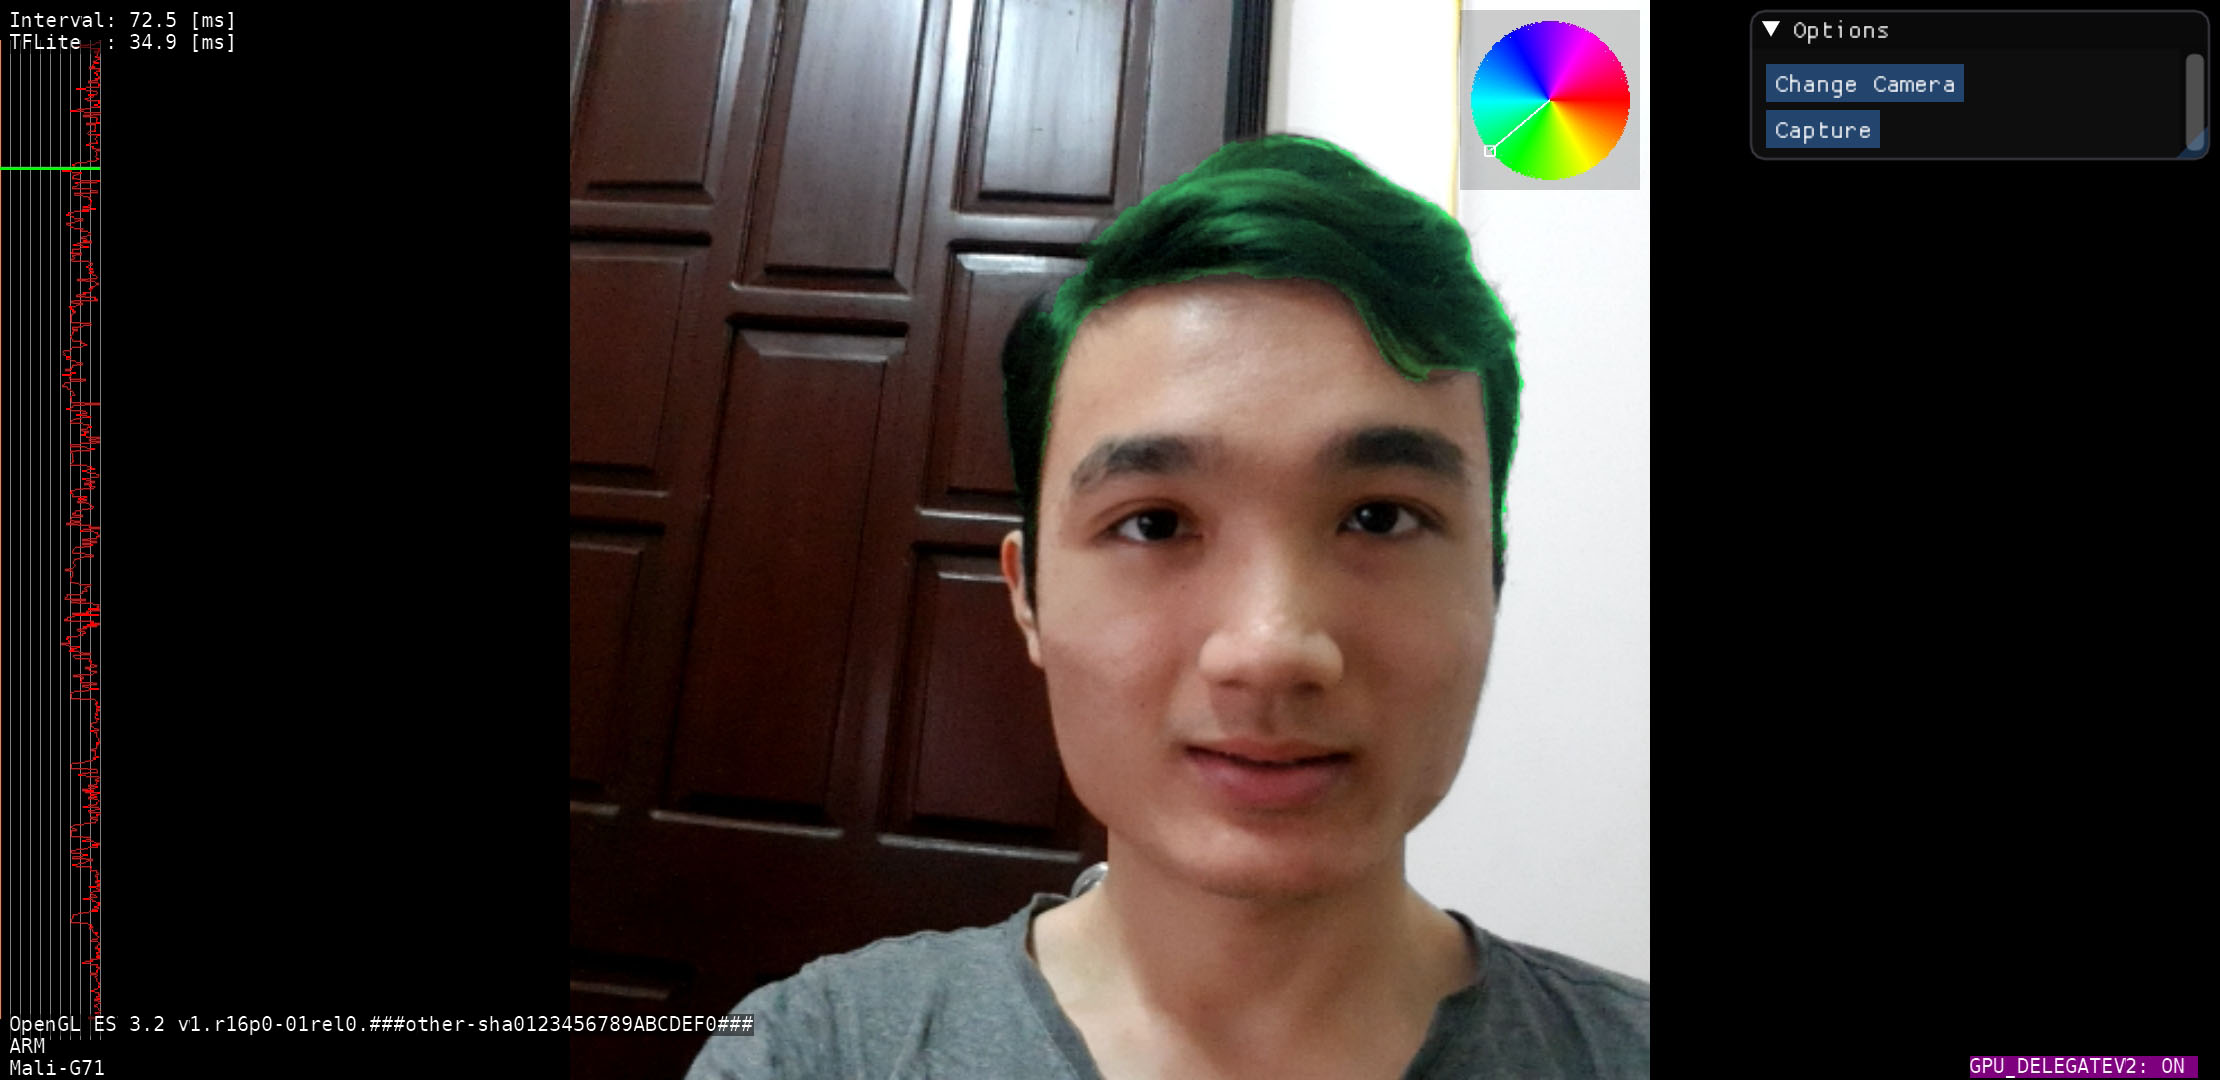
\includegraphics[width=0.7\textwidth]{chapter4/image/scanning.jpg}
    \caption{Illustration for Hair Color Scanning Activity}
\end{figure}


\begin{figure} [H]
    \centering
    \captionsetup{justification=centering}
    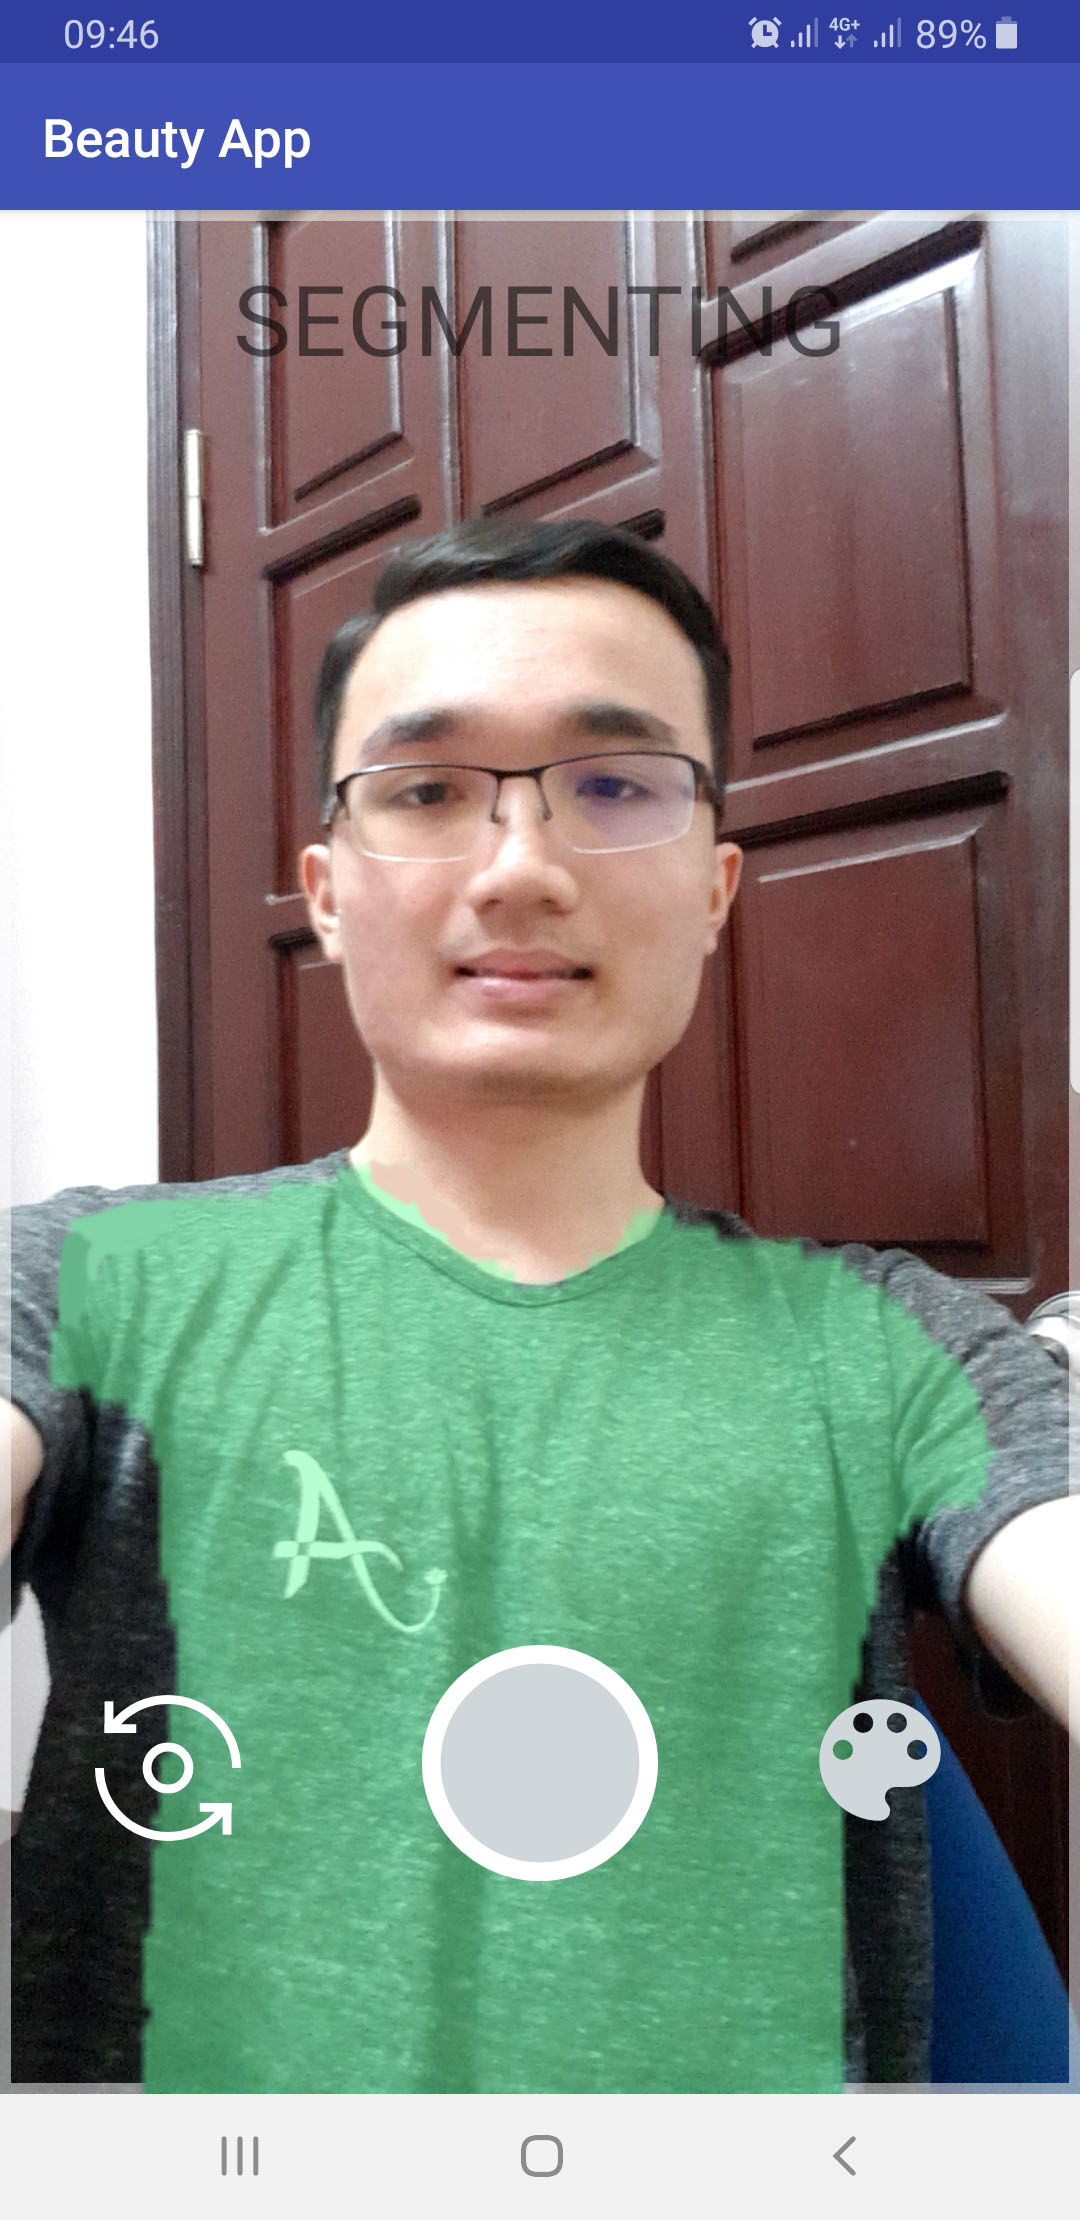
\includegraphics[width=0.3\textwidth]{chapter4/image/camerascreenshot.jpg}
    \caption{Illustration for Clothes Camera Activity}
\end{figure}




\subsubsection{Performance}
Because responsiveness is one of the most important non-functional requirements of the app, the performance is carefully evaluated. It is true that ML apps spend most of their execution time making predictions and rendering these predictions after that. Therefore, I take a measurement of the rendering speed of the two proposed rendering methods, apart from the inference speed of the two proposed models. To do that, I apply methods one by one into a specific use case and collect the results afterward. \par
 
This experiment is conducted on the Samsung S8+, having an ARM Mali-G71 GPU, 4 GBs of memory. The two following tables show the experimental results.

\begin{table}[H]
\centering
\caption{Average inference time of the app} 
 \begin{tabular}{||c c||} 
 \hline
 Model & Inference time (ms) \\ [0.5ex] 
 \hline\hline
  Hair segmentation & 200\\ 
 Cloth segmentation & 240 \\ [1ex] 
 \hline
 \end{tabular}
\end{table}


\begin{table}[H]
\caption{Average rendering speed of the app} 
\centering
 \begin{tabular}{||c c||} 
 \hline
 Method & Rendering time (ms) \\ [0.5ex] 
 \hline\hline
  Bitmap & 43\\ 
 OpenGL & 21 \\ [1ex] 
 \hline
 \end{tabular}
\end{table}


\subsection{Models}

The two proposed models, one for hair and one for clothes, are adapted from the U-Net architecture, already presented in \textbf{section \ref{sec:model}}. The models are trained with the hyperparameters listed in \textbf{section \ref{sec:experiments}}. For hair segmentation models, it is trained for 46 epochs. With the clothes segmentation task, the model is trained for 15 epochs, but in the first 10 epochs, the base net is frozen, in the rest epochs, the base net is unfreezing. All models are tested in the same dataset that they were trained in. The below table shows the results:

\begin{table}[H]
\caption{Accuracy of the proposed models} 
\centering
 \begin{tabular}{||c c||} 
 \hline
 Model & IoU (\%) \\ [0.5ex] 
 \hline\hline
  Hair segmentation & 88\% \\ 
 Clothes segmentation & 84\% \\ [1ex] 
 \hline
 \end{tabular}
\end{table}

